\chapter{绪论}
\label{chapter:Introduction}

\section{研究背景及意义}

可再生能源在世界范围内已经成为主流能源。可再生能源,尤其是清洁电力的快速发展,受到诸多因素的推动,包括可再生能源技术成本的降低,政府专项政策的出台,融资渠道更加完善,能源安全和环境问题的出现,发展中国家和新兴经济体对能源需求的不断增长,以及获得现代能源的需求。

太阳能因具有分布广泛,能量巨大,取之不竭,安全环保等优点,受到很多国家的关注,被认为是化石能源的最佳潜在替代者。国际能源机构预计,到2050年“大量应用可再生能源”的情景下,太阳能光伏发电量和太阳能光热发电量将分别占全球总用电量的16\%和11\%,太阳能将成为全球最大的电力来源\cite{IEA2014}。

太阳能光热发电是除太阳能光伏发电之外的另一种太阳能发电技术。由于太阳能能量密度较低,为了提高可用的能量密度,太阳能光热发电通常采用集热器(collector)来聚光集热发电,使用反射镜(reflector)将太阳光会聚到用于吸收太阳能的接收器(receiver)上,产生热量并将其传递给合成油、熔融盐或空气等传热流体。然后,传热流体直接或间接地为动力循环系统提供热量。
与太阳能光伏发电相比,太阳能光热发电因其能量密度高,发电平稳,电网兼容性好,易于与现有火力发电厂集成等优点受到越来越多的关注。

不同的太阳能光热发电技术使用不同种类的反射镜将太阳的光能会聚到接收器上并将其转换成热量。
现有三种已商业应用的CSP(聚光集热发电)技术:太阳能槽式发电,太阳能碟式发电和太阳能塔式发电。
图\ref{fig:collectors}展示了这三种CSP技术的应用实例。
\begin{figure}[!ht]
\centering
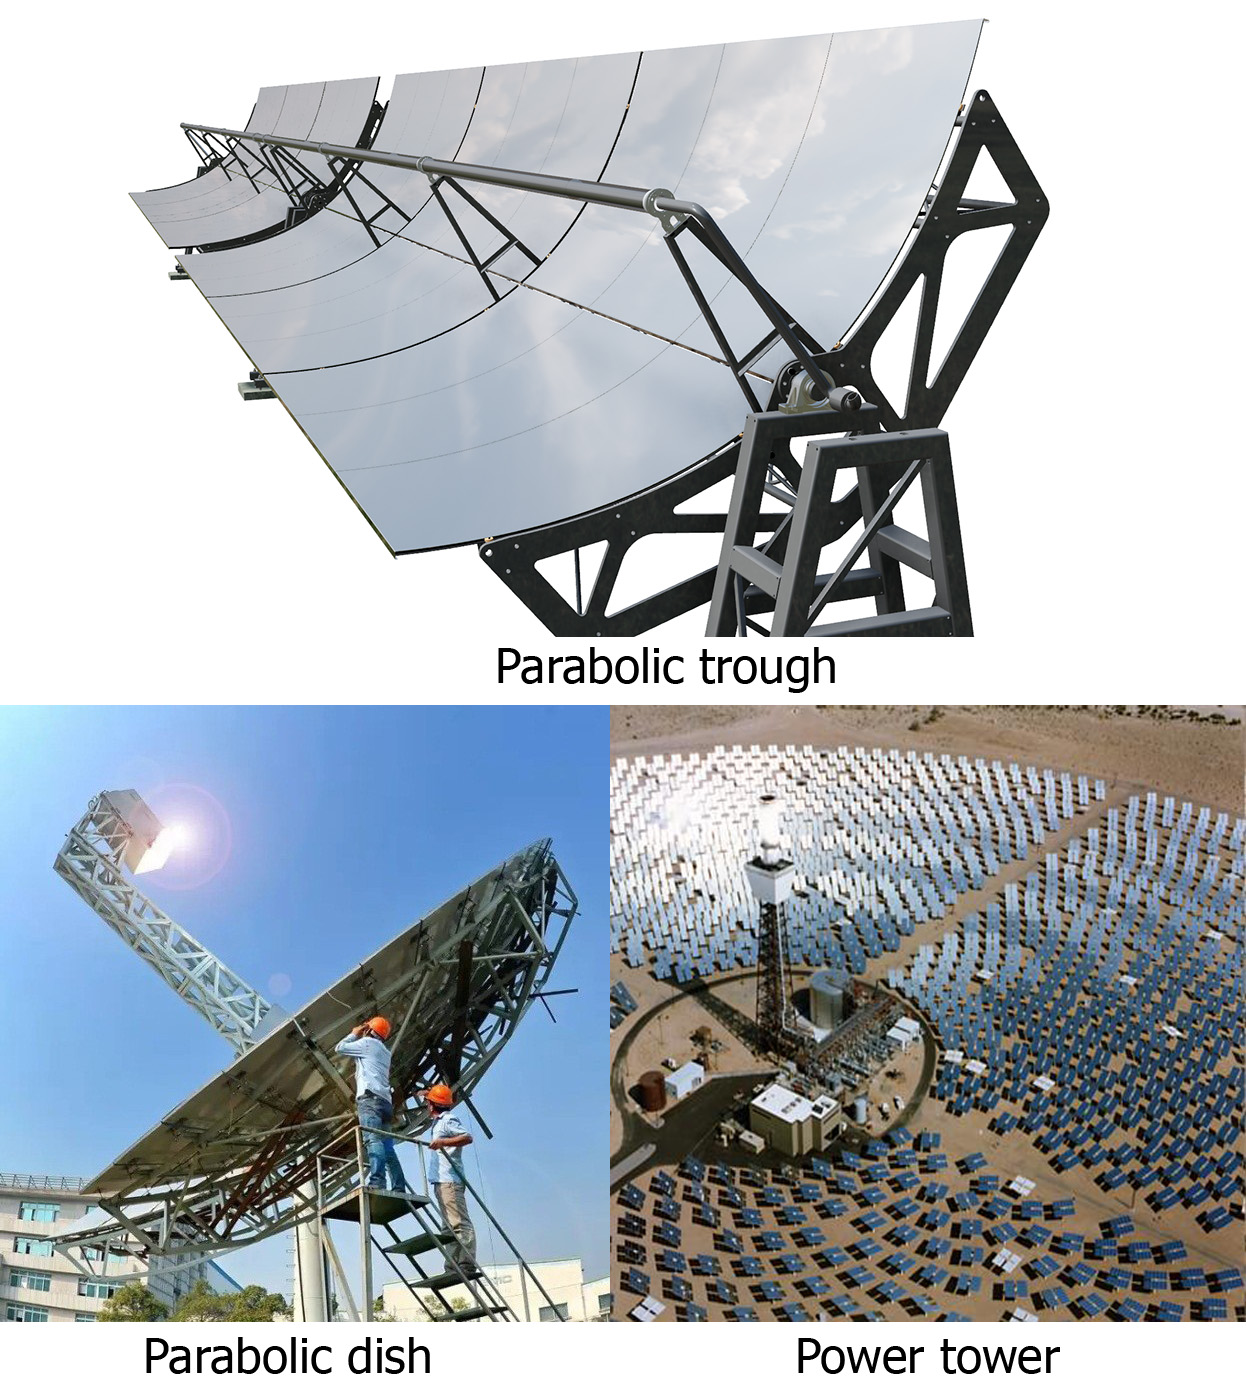
\includegraphics[width=.8\textwidth]{fig/Collectors}
\caption{三种CSP技术的应用实例}\label{fig:collectors}
\end{figure}

太阳能槽式发电的反射镜是槽型抛物面,反射镜在白天采用单轴跟踪的形式跟踪太阳。反射镜将太阳光反射聚集到位于焦线处的吸热管(absorber)上。传热流体(例如合成油)流经吸热管并吸收由聚集的太阳光产生的热量,提供给发电系统。
 
太阳能碟式发电的反射镜是旋转抛物面,它可以将沿着轴线照射的太阳光会聚到焦点上。碟式集热发电采用双轴跟踪系统来保证反射镜始终正对太阳从而避免了余弦损失。它可以拥有很高的聚光比,并因此获得高温热源。
通常情况下,焦点处放置有接收器或斯特林机来吸收会聚的能量。

太阳能塔式发电是一种使用位于高塔顶部的接收器来接收聚集阳光的太阳能发电技术。它使用大量可移动的太阳能反射镜(称为定日镜),每台定日镜都各自配有跟踪机构将太阳光实时准确地反射到位于塔顶的接收器上。该跟踪机构为双轴跟踪(从东向西,向上和向下)跟踪太阳。接收器吸收集中的太阳辐射将太阳能转换成热量,再被传热流体传递至热力循环系统用于发电。

在三种太阳能光热发电技术中,太阳能槽式发电是最成熟和最具商业化的技术。但是,它的聚光比比较低,接收器的集热温度比较低,光热发电效率也比较低。太阳能碟式发电的聚光比高达数百甚至数千,因此可以获得高温热能,其光热发电效率高于太阳能槽式发电。此外,太阳能碟式发电的一个优点是它的发电过程用水量非常少。然而,太阳能碟式发电并未实现大规模应用,其结构紧凑,安装方便,主要应用于分布式发电。当使用大量的定日镜时,太阳能塔式发电的塔顶会聚了大量的能量,接收器可以达到很高的温度,而且太阳能塔式发电也可以实现大规模应用。但与此同时,它也具有投资高,系统复杂度高的缺点。太阳能塔式发电目前处于快速发展阶段。

不同种类的太阳能光热发电技术具有各自的优缺点,找到一种能够利用现有太阳能光热发电技术的优势并克服其缺点的方法在大力发展太阳能发电的时代背景下显得额外重要。换句话说,开发出一种效率更高,成本更低的新的太阳能光热发电技术迫在眉睫。
本文试图通过提出使用不同型式的太阳能集热器和不同种类的热力循环的梯级系统来实现这一目标。这可能是实现大规模高效率低成本太阳能光热发电的新的可行技术。

\section{国内外研究现状}

\subsection{太阳能槽式发电}

太阳能槽式发电技术是目前最成熟成本最低的大规模太阳能光热发电技术\cite{Price2002}。许多研究人员做了大量的工作来研究太阳能槽式发电,以提高性能或降低成本。其中很多研究为旨在测试抛物槽接收器的热力性能和机械性能的实验性工作。

来自桑迪亚国家实验室的Dudley等人\cite{Dudley1994}测试了应用于SEGS太阳能光热电站的LS-2型槽式接收器的集热效率和热损失。实验分析了不同类型的选择性涂层,不同接收器配置,不同真空度对集热器性能的影响。还建立了槽式接收器的一维分析模型,并将模拟结果与实验数据进行了对比分析。

来自美国国家可再生能源实验室的Burkholder和Kutscher\cite{Burkholder2009}测试了产自Solel公司的UVAC3型槽式集热器和产自Schott公司的PTR70型槽式集热器,并建立了以接收器平均温度和环境温度为参数的热损失方程。

Kr\"uger等\cite{Kruger2008}对Solitem PTC 1800型槽式集热器的光学性能进行了研究,并以工作温度为200$^\circ\mathrm{C}$的高压水作为传热流体进行了实验分析,对光学效率的改进提出了建议。

Reddy等\cite{Reddy2015b}开发并研究了六种不同型式的槽式接收器,并进行了性能对比分析。依据ASHRAE 93-1986测试程序,对一台集热面积为15$\,\mathrm{m^2}$的集热器的六种不同型式的接收器进行了实验测试分析。实验表明,多孔圆盘型接收器可以显著提高槽式集热器的性能,可以有效地用于工业加热过程。

%众所周知,实验研究最具有说服力和可信性,然而,实验研究需要大量的研发成本和实验时间,所以槽式太阳能光热发电的大部分工作都采用模拟分析的方法,通过建造相关模型,对槽式集热器进行研究,或是通过实验对所建立的模型及方法进行相关的验证工作。

一些研究人员研究了槽式集热器的光学效率模型。王金平等\cite{Wang2016}提出了用于计算槽式集热器的光学效率的数学模型,并选取了中国的三个典型地区作为实验地点,进行了相关的实验验证工作。结果表明,其提出的光学效率数学模型的相对误差在1\%到5\%之间。
邹斌等\cite{Zou2017}研究了太阳形状和入射角对槽式集热器的性能影响,发现太阳形状对光学效率具有很大的影响,需要在实际应用中考虑此因素。更宽的集热器开口和更细的吸热管将使入射角对端部损失的影响更大。此外还发现,对于特定集热器存在着最佳焦距使光学效率获得最大值。
L\"upfert等\cite{Lupfert2006}介绍了实际工程应用中用于分析槽式集热器的形状参数和光学参数的技术,并对槽式集热器的集热器形状测量、光通量测量、光线跟踪、热性能分析等的数据进行了分析。结果表明,不同的测量方法和参数分析可以获得一致的结果,这些结果可以为下一代测量技术和分析方法提供参考。
许成木等\cite{Xu2014}分析了南北布置的槽式集热器的光学效率,提出了一种补偿端部损失的方法,推导出了端部损失比例与采用补偿损失方法后效率增加量之间的计算公式。计算分析了不同纬度的日光学损失率,年光学损失率,以及采用补偿损失方法后的日增光学效率和年增光学效率。结果表明,该补偿方法对于纬度高于25度的地区的短集热器非常适用。
黄卫东等\cite{Huang2012}提出了一种新的光学性能分析模型,该模型采用了改进的积分算法,用于模拟带有真空管的槽式接收器的性能。首先推导了反射镜各点光学效率的解析方程,然后用数值积分算法模拟了系统的光学效率。可以通过该程序计算出余弦损失,集热效率和热损失。

一些学者对槽式系统进行了热效率和㶲效率分析,试图从能量利用的数量和品质上提升槽式系统的性能。
Padilla等\cite{Padilla2014}在其建立的传热模型\cite{Padilla2011}的基础上进行了㶲效率分析,来研究实验操作和环境参数对槽式集热器性能的影响。分析考虑了传热流体的入口温度,质量流量,风速,真空压力以及太阳法向直射强度等因素。结果表明,传热流体的入口温度,太阳法向直射强度和真空度对散热性能有显著影响,但传热流体的流量和风速的影响很小。如果传热流体入口温度固定,则不能同时获得最大的热效率和㶲效率,二者呈现相反的变化趋势。最后,还发现最大㶲损发生在接收器与太阳之间的辐射传热过程中。
郭江峰等\cite{JiangfengGuo2016-1}研究了各种参数对槽式集热器的热效率和㶲效率的影响。结果发现,随着传热流体的质量流量,环境温度和入射角的增大,太阳能接收器的热损失随之减少。随着传热流体入口温度,风速和玻璃管内径的增加,槽式接收器的㶲损失也随之增加。当入射角较大时,存在最佳的传热流体流量使㶲效率获得最大值。

一些研究人员致力于使用新方法开发出精度更高的槽式系统模型。Behar等\cite{Behar2015}开发并验证了一种新颖的槽式集热器模型。通过与桑迪亚国家实验室和国家可再生能源实验室建立的模型进行比较,该模型显示出更好的集热效率预测精度。
Padilla等\cite{Padilla2011}针对槽式集热器建立了详细的一维数值分析模型。为了求解换热过程中的数学模型,偏微分方程被离散化,然后通过求解非线性代数方程得到槽式集热器的数值分析结果。该模型得到的数值结果利用桑迪亚国家实验室的实验数据进行了验证。
Hachicha等\cite{Hachicha2013}基于有限体积法建立了详细的一维槽式集热器模型。该模型还采用了光线追踪法,考虑了太阳大小带来的影响。该模型通过文献上的数据进行了验证,和其它模型及实验结果具有很好的一致性。
郭江峰与淮秀兰\cite{JiangfengGuo2016-2}基于基因算法对槽式接收器进行了多目标参数优化研究,该研究同时以热效率和㶲效率为优化目标。
Boukelia等\cite{Boukelia2016}研究了三种应用于的人工神经网络的不同形式的前馈向后传播学习算法,包括Levenberge Marguardt法、扩展共轭梯度法和Pola-Ribiere共轭梯度法,并利用这些算法对槽式电厂进行预测和技术经济优化分析。
刘启斌等\cite{Liu2012}开发了基于LSSVM(最小二乘支持向量机)方法的槽式集热器模型并通过数值模拟评估了LSSVM方法的有效性。
Lobon等\cite{Lobon2014}引入了计算流体动力学特性的模拟方法来模拟槽式系统中的蒸汽发生系统,该蒸汽发生系统位于西班牙Plataforma Solar de Almeria。利用CFD(计算流体动力学)代码包STAR-CCM+建立了一个有效的多相流体模型,可以模拟槽式集热器中的多相流体的动力学行为。模拟结果和实验数据在各种工作条件下进行了对比分析。
为了得到槽式集热器的动力学特性,并计算出散热损失,Mohamad等\cite{Mohamad2014}分析了工作流体,吸热管和玻璃管沿轴向的温度分布。结果发现,使用双层玻璃罩可以有效提高高温运行时的集热效率。然而,当集热器的长度小于10$\,\mathrm{m}$时,使用单层玻璃罩比双层玻璃罩更经济。结果还清晰地表明,随着吸热管管径的增大,热损失迅速增加。
郭苏等\cite{SuGuo2016}针对槽式系统中的直接蒸汽发生系统开发了一个非线性分布的参数模型来模拟在全部或部分太阳辐射干扰下的直接蒸汽发生系统的动态特性。该模型具有两个优点:(1)传热系数和摩擦阻力系数采用实时局部值;(2)考虑了接收器的完整回路,包括过冷区,蒸发区和过热区。该模型使用新南威尔士大学太阳能热能实验室的实验数据进行了验证,出口流体温度相对误差仅为1.91\%。

一些研究人员还提出了新的太阳能槽式系统。Ashouri等\cite{Ashouri2015}将一台小型槽式集热器,一台蓄热罐和一台辅助加热器连接到一个卡林那循环,并分析了其全年热力性能和全年经济性能。

Good等\cite{Good2016}提出了使用空气作为槽式集热器的传热流体的集热方案,空气的集热温度可达600$\mathrm{^\circ C}$。吸热管由一组螺旋卷曲的金属管组成,外层包裹着矩形截面的绝缘槽。该方案采用二次反射镜面将聚光比提升至97。
Bader等\cite{Bader2015}针对采用空气作为传热介质的槽式真空接收器建立了数值模型。该模型考虑了四种不同的接收器型式,包括光滑圆管吸热管和V型吸热管,单层套管和双层套管。该数值模型考虑了不同类型的热损失以及吸热管内的温度分布。
Kaloudis等\cite{Kaloudis2016}利用CFD软件对采用含有纳米颗粒的流体作为传热介质的槽式集热器进行了模拟分析。该模拟使用Syltherm 800作为流体,在其中加入了浓度为0\%到4\%的氧化铝纳米颗粒。结果发现,当纳米颗粒浓度为4\%时,系统的集热效率可以获得10\%的提升。

Al-Sulaiman等\cite{AlSulaiman2012}基于槽式集热器和有机工质朗肯循环提出了一种冷热电三联供的新型系统,并对系统的效率、电功率、供热供冷比进行了性能评估。研究表明,该系统对于发电,太阳能模式最高效率可达15\%,太阳能和蓄能联供模式为7\%,只使用蓄能模式为6.5\%。对于冷热电三联供,太阳能模式的最高效率为94\%,太阳能和蓄能联供模式为47\%,只使用蓄能模式为42\%。
%\nomenclature[C]{CCHP}{Combined cooling, heating and power}
%\nomenclature[C]{HTF}{Heat Transfer Fluid}
\nomenclature[C]{CFD}{计算流体动力学}
%\nomenclature[C]{DSG}{直接生产蒸汽系统}
%\nomenclature[C]{LM}{Levenberge Marguardt}
%\nomenclature[C]{SCG}{Scaled Conjugate Gradient}
%\nomenclature[C]{PCG}{Pola-Ribiere Conjugate Gradient}
%\nomenclature[C]{ANN}{Artificial neural network}

\nomenclature[C]{SRC}{水工质朗肯循环}
\nomenclature[C]{ORC}{有机工质朗肯循环}
%\nomenclature[C]{PTC}{Parabolic Trough Collector}
%\nomenclature[C]{SNL}{Sandia National Laboratory}
\nomenclature[C]{LSSVM}{最小二乘支持向量机}

\subsection{太阳能碟式发电}
\label{sec:pd}

太阳能碟式发电系统因其在所有太阳能技术中具有最高的光电转换效率(约30\%)而为人所知,其因结构紧凑并且易于安装而主要应用于分布式发电系统。

许多研究人员致力于通过实验探究太阳能碟式发电系统或者用于验证提出的模型。
为了探究适用于太阳能碟式系统的半球形腔体式接收器的热损失,谭雨亭等\cite{Tan2014b}通过实验研究不同工质入口温度,接收器倾角和开口大小对接收器效率的影响。实验结果导出了以格拉晓夫数为函数的努塞尔数的关联式。
Chaudhary等\cite{Chaudhary2013}探究了使用碟式接收器的太阳炉,该太阳炉采用PCM(相变蓄热材料)存储吸收的热量。探究过程使用三个案例:普通太阳炉,外表面被涂黑的太阳炉和外表面涂黑且上釉的太阳炉。结果表明最后一个案例具有最佳性能,与前两个案例相比,能分别为PCM系统多存储32.3\%和26.8\%的热量。
Mawire和Taole\cite{Mawire2014}探究了应用于SK-14型碟式聚光镜的圆柱形腔体式接收器的集热性能。结果发现,接收器的㶲效率明显低于能量效率。在较高太阳辐射强度条件下,该聚光碟系统的光学效率约为52\%。
朱剑琴等\cite{Zhu2015}通过实验来探究管式太阳能碟式接收器。当太阳法向直射强度约为650$\,\mathrm{W/m^2}$时,采光口处的太阳能能量密度约为1000$\,\mathrm{kW/m^2}$。对接收器进行了能量分析和㶲分析,结果表明,在稳定状态下,能量效率维持在80\%,㶲效率约为28\%。
CRTEn(Borj Cedria能源研究与技术中心)组建了一个太阳能碟式系统,并使用四种吸热器进行了实验研究。这四种吸热器包括:平板式,圆盘式,热量计式和太阳能换热器式。对于不同类型的吸热器,通过实验得到平均聚光比,能量效率和㶲效率。结果表明系统的热效率在40\%到77\%之间,聚光系统的平均㶲效率在50\%左右,聚光比在178左右。
Thirunavukkarasu等\cite{Thirunavukkarasu2017}通过实验来探究腔体式碟式集热器的接收器的集热性能。集热器的整体热效率是69.47\%。接收器的平均㶲效率为5.88\%,峰值㶲效率为10.35\%。
Pavlovic等人\cite{Pavlovic2017}进行了碟式太阳能系统的实验研究。该系统中使用了不同工质(水,导热油和空气)来验证了利用EES建立的数值模型。结果表明水最适用于低温工况,而导热油最适用于高温工况。

一些研究者关注于碟式聚光器,许多人提出不同形状的聚光器。完美的聚光器是旋转抛物面型反射镜,但实际上,很多碟式聚光器由多片弧形镜面组成,这是由诸多因素(易于加工,运输安全,成本低廉等)导致的。SG3由澳大利亚国立大学在1994年设计并建造,是一个具有400$\,\mathrm{m^2}$反射面积的大型碟式太阳能聚光器,其实物图如图\ref{fig:LargeDish}所示\cite{Lovegrove2011}。SG3系统成功地证实了一个比其它任何聚光器大将近三倍的聚光器的技术可行性。
\begin{figure}[!ht]
\centering
\includegraphics[width=.8\textwidth]{fig/largeDish.jpg}
\caption{澳大利亚国立大学的400$\,\mathrm{m^2}$反射面积的SG3碟式系统}\label{fig:LargeDish}
\end{figure}
Berumen等人\cite{Berumen2004}建造了一个由12个玻璃纤维制成的镜面组成的反射器。这些镜面的反射面由反射率为86\%的铝薄膜制成。
Pavlovic等\cite{Pavlovic2014}开发了一段程序用于描述实验室规模的抛物面型聚光器中温集热的热力学过程。该聚光器由多块独立方形镜面组成。这些镜面能够将高达13.604$\,\mathrm{kW}$的辐射能量以平均超过1200的聚光比传输到半径为250$\,\mathrm{mm}$的碟式接收器中。
Hijazi等\cite{Hijazi2016}设计了一个低成本的碟式太阳能聚光镜。该聚光镜由多片中小型号的反射镜组成,这些反射镜的形状尺寸都经过了精心的设计。
马宏财等\cite{Ma2012}设计了一个基于三角形薄膜面的太阳能碟式聚光器。该聚光器由600个焦距直径比为1.1的薄膜面组成,焦点平面上放置有半径为15$\,\mathrm{cm}$的圆盘。该聚光集的太阳辐射能收集效率可达83.63\%,平均聚光比超过300。
桑迪亚国家实验室\cite{Schertz1991}成功设计并制造了一个直径为3.6$\,\mathrm{m}$的薄膜拉伸反光面。十二个相同的反光面被用于组成碟式集热器的轻型反射面。项目目标是实现任意两个全尺寸反光面之间的表面精确度小于2.5$\,\mathrm{mrad}$,目前的原型精确度已经可以低至1.1$\,\mathrm{mrad}$。

许多研究者探究了太阳能碟式接收器的热流密度分布和热力学性能。Shuai等\cite{Shuai2010}建立了一个为碟式聚光器测量热流密度分布的系统。应用了CCD(电荷耦合装置)照相机在不同目标位置获得热流分布的云图。然后,将测量的热流分布与通过蒙特卡罗方法预测的分布进行对比分析。其结果可为设计和装配太阳能收集系统提供重要参考。
毛前军等\cite{Mao2014b}通过MCRT(蒙特卡罗光线追踪)法模拟了一个碟式接收器的热流密度分布,探究了太阳辐射强度,长径比(接收器高度与接收器直径之比)和系统误差对于接收器辐射热流的影响。
李志刚等\cite{Li2011b}使用MCRT法来研究太阳能碟式接收器的辐射热流分布。获得的结果在通过实验验证之后,作为CFD接收器模型的边界条件。数值模拟考虑了吸热器内流体流动与热传递的耦合,其结果经过了实验验证。
Wang和Laumert\cite{Wang2017}使用光线追踪法来研究腔体表面材料对于冲击型接收器的热流分布的影响,研究了五种表面材料及它们制成的接收器。结果表明,相比于圆柱底面材料,热流分布和总光学效率对圆柱侧面材料更敏感。
Blazquez等\cite{Blazquez2016}研究了碟式系统的聚光器和接收器的几何优化。使用了开源软件Tonatiuh(一款专门利用MCRT法进行光线追踪的太阳聚光器建模工具)对其进行光线追踪分析。
Reddy等\cite{Reddy2015,Reddy2015b}对一个改进型的腔体式接收器进行了热力学性能理论研究,该接收器对应的聚光镜为模糊焦点式的碟式聚光镜。在评估该改进型腔体式接收器的总热损时,考虑了风力条件、运行温度、腔体表面发射率和绝缘层的厚度等条件的影响。实施定时测试的方法来应对太阳辐射强度产生突变对稳态运行的影响,并针对不同流量条件下的日常性能进行了测试。
Vikram和Reddy\cite{Vikram2015}使用三维数值模型来探究采用三种配置的碟式接收器的腔体的总热损。探究了腔体长径比、倾角、运行温度、绝热层厚度和发射率对于腔体热损失的影响。基于人工神经网络模型,为对流、辐射和总热损的计算提出了一个修正后的努塞尔数关联式。

一些研究人员专注于研究碟式系统的太阳跟踪系统。
Patil等\cite{Patil2016}描述了其开发碟式太阳能光热系统的双轴自动跟踪系统的过程。测试了五种用于检测阳光的光敏电阻器,两种用于移动聚光碟的永磁体直流电机,并最终开发出了控制软件来利用光敏电阻器的数据控制电机实现跟踪。
Raturi等\cite{Raturi2014}提出一个基于重力而不需要任何额外能量的太阳跟踪系统。样机测试结果和分析表明这个系统可以成功运行。
邝坚和张威\cite{Kuang2012}开发了新的跟踪系统的设计和安装方法,来改进基于主动跟踪和被动跟踪的嵌入式系统的跟踪精度。
金小山等\cite{Jin2013}描述了一种带有PLC(编程逻辑控制器)的双轴太阳跟踪系统和一种更高精度的结合了主动和被动跟踪方法的混合跟踪方法。
Shanmugam和Christraj\cite{Shanmugam2005}针对碟式集热器提出了一种间歇性跟踪方法,这种方法只考虑南北方向的跟踪而不考虑东西方向的跟踪,以减少跟踪过程的能量消耗。南北方向的跟踪动作频率由太阳高度角和碟式集热器的吸热器的尺寸决定。
\nomenclature[C]{MCRT}{蒙特卡洛光线追踪}
\nomenclature[C]{PLC}{编程逻辑控制器}
%\nomenclature[C]{CRTEn}{Borj Cedria能源研究与技术中心}

\subsection{太阳能塔式发电}
\label{sec:st}

太阳能塔式发电技术因其规模大,聚光比高,运行温度高而日益受到关注。它被广泛认为是最有前景的太阳能光热发电技术。

太阳能塔式发电技术的优势之一在于部件易于更新及系统便于改进。所以不同的研究者专注于塔式技术的不同领域。
一些研究者专注于太阳能塔的工质选择。
一些已经标准化的商业电站采用传统的水工质朗肯循环\cite{Spiros2017}。水在朗肯循环中被同时用作传热工质和做功工质。在接收器中直接产生蒸汽,流入汽轮机膨胀做功发电\cite{Montes2009,Feldhoff2012,Steinmann2006,Yu2017,Gonzalez2017}。许多研究者致力于研究使用其他流体(熔融盐,空气等)作为传热工质。
Toto等\cite{Toro2016}提出了一种在顶部使用空气介质的布雷顿循环和底部使用朗肯循环发电的太阳能塔的概念。
Rold\cite{Rold2016}提出一种理想的使用超临界CO$_2$作为传热流体的太阳能塔。建立了一个简化的CFD模型来分析以超临界CO$_2$作为传热流体的太阳能塔的可行性。结果表明这可以获得更好地运行条件和更低的维护成本。
Joshi等\cite{Joshi2016}使用动力学模拟技术评价了一个采用熔融盐为传热流体的中心接收器的设计及其控制策略。

许多研究者关注定日镜在有风载荷和热应力条件下的跟踪精度问题,另一方面,在更高土地利用率和更低遮挡系数之间取得平衡也是研究的热点问题。
Thalange等\cite{Thalange2017}提出了三脚架定日镜系统结构分析的方案,以降低成本并提高机械性能。
Besarati和Yogi\cite{Besarati2014}开发了一种新的简单的方法来提高计算定日镜场的阴影和遮挡分析的速度和精度。该方法使用了Sassi法\cite{Sassi1983}来计算阴影率和遮挡率。美国加利福尼亚州Dagget的50$\,\mathrm{MW}$的定日镜场被用来作为本方法应用的研究案例。
魏秀东等\cite{Wei2010}为太阳能塔式电站的定日镜场的布置设计提出一种新型的方法。基于这种新方法开发了针对定日镜场布置设计的代码,并且使用该代码为PS10电站进行了镜场布置设计。与现行的PS10布置方案相比较,新设计的布置方案能保证定日镜在相同光学效率的条件下具有更高的响应速度。
并开发出了一种新的简单的方法来提高计算定日镜场的阴影和阻挡影响的计算速度和精度。

一些研究者关注塔式电站中心接收器的性能。
Kim等\cite{Kim2015}研究了太阳能中心接收器的热损失。使用CFD进行数值模拟研究了四种不同形状的接收器的对流损失和辐射损失。在模拟中考虑了不同腔体开口面积比(开口面积与腔体截面面积之比),接收器温度,风速和风向(正面迎风和侧面迎风)的影响,得到了对流损失的简化关系式的模型。该关系式已被三个中心接收器系统(Martin Marietta,Solar One和Solar Two)的实验数据所证实。
Lara等\cite{Lara2016}开发了新颖的建模工具来计算分析中心接收器聚光热流分布情况。该建模工具基于漂移模型,该模型以严格的方式包含了不同的几何误差源,并且对单个定日镜的通量分布进行了简单的近似分析。

许多研究者致力于塔式电站的模拟工作。
Franchini等\cite{Franchini2013}开发了用于分析太阳能塔式系统在满负荷和部分负荷工况下运行特性的计算程序。将西门子SGT-800型燃气轮机应用于ISCC(综合太阳能联合循环)系统作为太阳能塔式系统的研究案例。该燃气轮机拥有双压力热回收蒸汽发生器,可用于整合ISCC系统。此外还开发了一个由太阳能塔驱动的太阳能朗肯循环模型用于比较。结果发现,设计的ISCC装置可以达到21.8\%的光电转换效率。在所有情况下,ISCC的整体光电转换效率都高于太阳能朗肯循环模型。
徐二树等\cite{Xu2011a,Xu2012}利用模块化建模方法构建了1$\,\mathrm{MW}$的Dahan塔式太阳能电站的模型。基于该模型,分析了电站的动态特性和静态特性,给出了不同太阳辐射强度下的相关系统状态参数曲线。该文献可为塔式太阳能电站的设计提供良好的参考依据。
Benammar等\cite{Benammar2014}为塔式太阳能电站开发了一个基于能量分析的数学模型。针对所研究系统的一般非线性数学模型,用数值优化方法进行了求解。结果表明,对于不同的蒸汽质量流量,接收器表面温度和接收器表面积都存在最佳的接收器效率值。
\nomenclature[C]{ISCC}{综合太阳能联合循环}

\subsection{太阳能梯级集热发电}
\label{sec:cs}

为了更加有效地利用太阳能光热发电系统中各部件的特性,许多研究人员研究了梯级太阳能系统。梯级太阳能系统的研究主要有两个方向:一个是梯级收集,一个是梯级利用。

\subsubsection{梯级收集}

许多研究人员研究了在太阳能光热发电技术中采用多种集热器实现太阳能梯级收集的方案。Suzuki\cite{Suzuki1986}分析了使用两种不同型式的集热器串联连接的集热方案。研究表明,集热器的一个参数值——集热效率和光学效率的乘积,是决定梯级系统是否比单独使用任何一种集热器更高效的关键参数。如果更低聚光比的集热器的这个参数值比更高聚光比的这个参数值大,那么梯级系统更加高效。此外还发现,梯级系统具有最佳的运行参数。

Kribus等\cite{Kribus1999}提出了多级独立开口的方案来利用太阳辐射的不均匀分布特性。传热流体依次经过辐射能量密度递增的接收器来实现逐级加热。为了验证这种方案,在魏茨曼研究所的太阳能塔的塔顶放置了一个双级接收器。在该接收器中,空气作为传热流体在低温级中被加热至750$\mathrm{^\circ C}$,然后流入高温级被加热至1000$\mathrm{^\circ C}$。该双级接收器的结构图如图\ref{fig:Kribus1999}所示。

\begin{figure}[!ht]
\centering
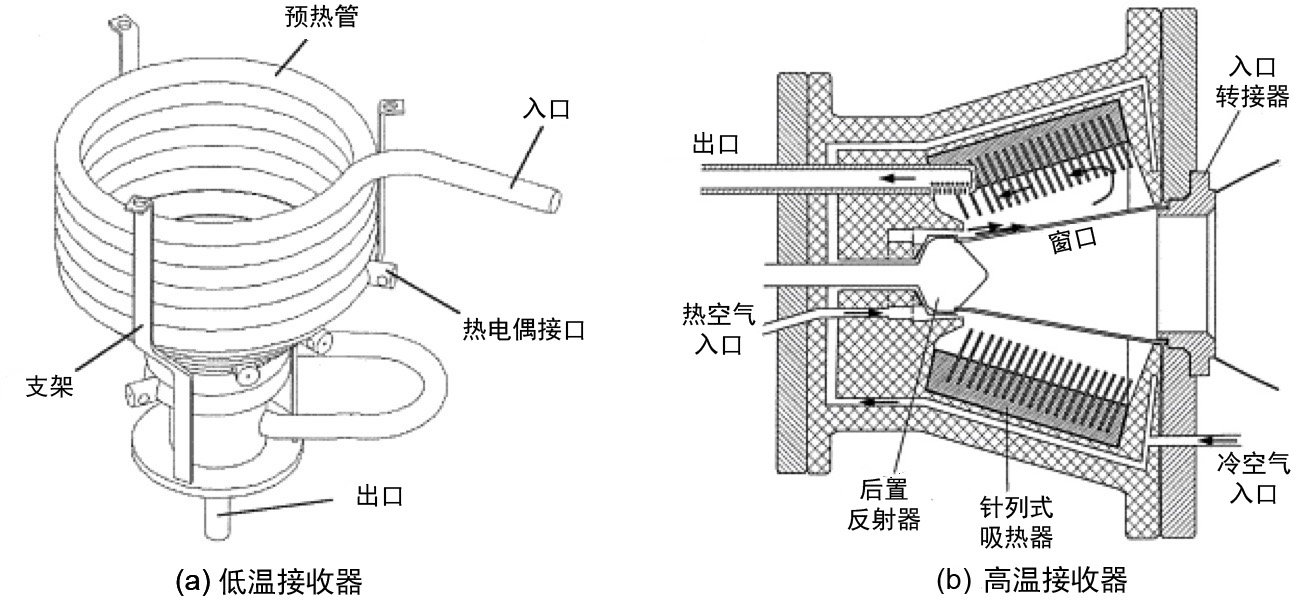
\includegraphics[width=.8\textwidth]{fig/Kribus1999.jpg}
\caption{双级集热器的结构图}
\label{fig:Kribus1999}
\end{figure}

Gordon和Saltiel提出了一种分析方法来预测采用多种型式集热器的光热系统(“多级”系统)的长期性能。该分析方法允许设计者针对给定负荷,来决定使用组合不同型式集热器的最有效的方法。一个成功的实例证明了该方法可以有效节省“多级”系统的成本。

Oshida和Suzuki\cite{Oshida1987}提出了利用不同类型集热器实现梯级集热的思想。梯级系统中使用两个吸热器,分为低温吸热器和高温吸热器,其中低温吸热器由菲涅尔镜片加热,高温吸热器由槽式镜面加热。传热流体先流经低温吸热器完成预热,再在高温吸热器中完成进一步加热。传热流体可以在该梯级系统中更加高效地完成加热过程。

Desai等\cite{Desai2015}提出了一种集成太阳能集热方案,该方案同时采用槽式集热器和线性菲涅尔集热器。该集成集热方案的系统结构图如图\ref{fig:Desai2015}所示。对采用集成集热方案的电厂进行了热力学和经济学分析,并同基于槽式集热器的电厂和基于线性菲涅尔集热器的电厂进行了对比。结果表明,采用集成方案的电厂的发电成本要比基于槽式集热器的电厂低9.6\%,比基于线性菲涅尔集热器的电厂低13.5\%。

\begin{figure}[!ht]
\centering
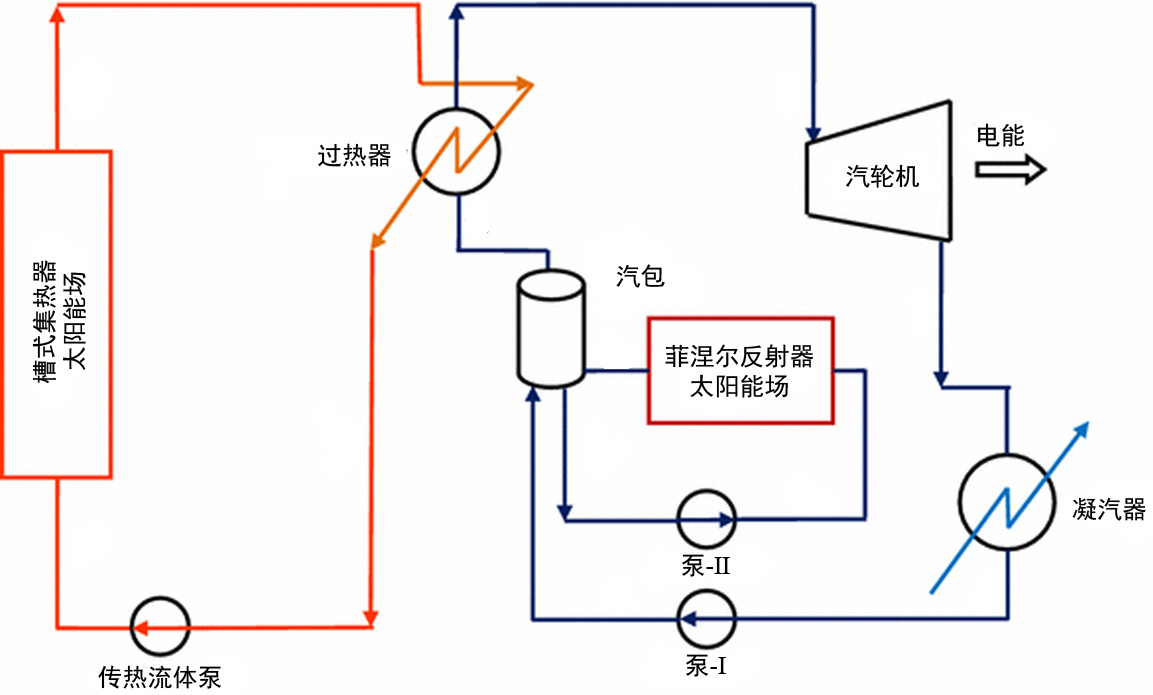
\includegraphics[width=.7\textwidth]{fig/Desai2015.jpg}
\caption{采用集成集热方案的系统结构示意图}\label{fig:Desai2015}
\end{figure}

Coco等\cite{Coco2015}为集成了直接蒸汽发生系统和布雷顿循环的系统提出了四种不同的线性集热太阳能光热发电方案。在这些方案中,太阳能场被分成了不同的片区来满足不同的集热需求。这种思想为在太阳能场中使用多种型式的集热器提供了可行性。

%\nomenclature[C]{CPC}{Compound parabolic collector}

\subsubsection{梯级利用}

很多学者致力于在太阳能光热发电系统中组合使用多种热力循环来实现能量的梯级利用。其中大部分的工作聚焦于ISCC,通常在联合循环中,朗肯循环作为底部循环,布雷顿循环作为顶部循环。

李元媛和杨勇平\cite{Li2014}提出了一种新颖的ISCC系统,可以实现高达30\%的光电转换效率,其系统结构图如图\ref{fig:Li2014}所示。分析了将收集到的太阳能用于ISCC系统不同位置对系统整体性能的影响后发现,将太阳能用于蒸发过程可以获得最大的系统整体性能。
\begin{figure}[!ht]
\centering
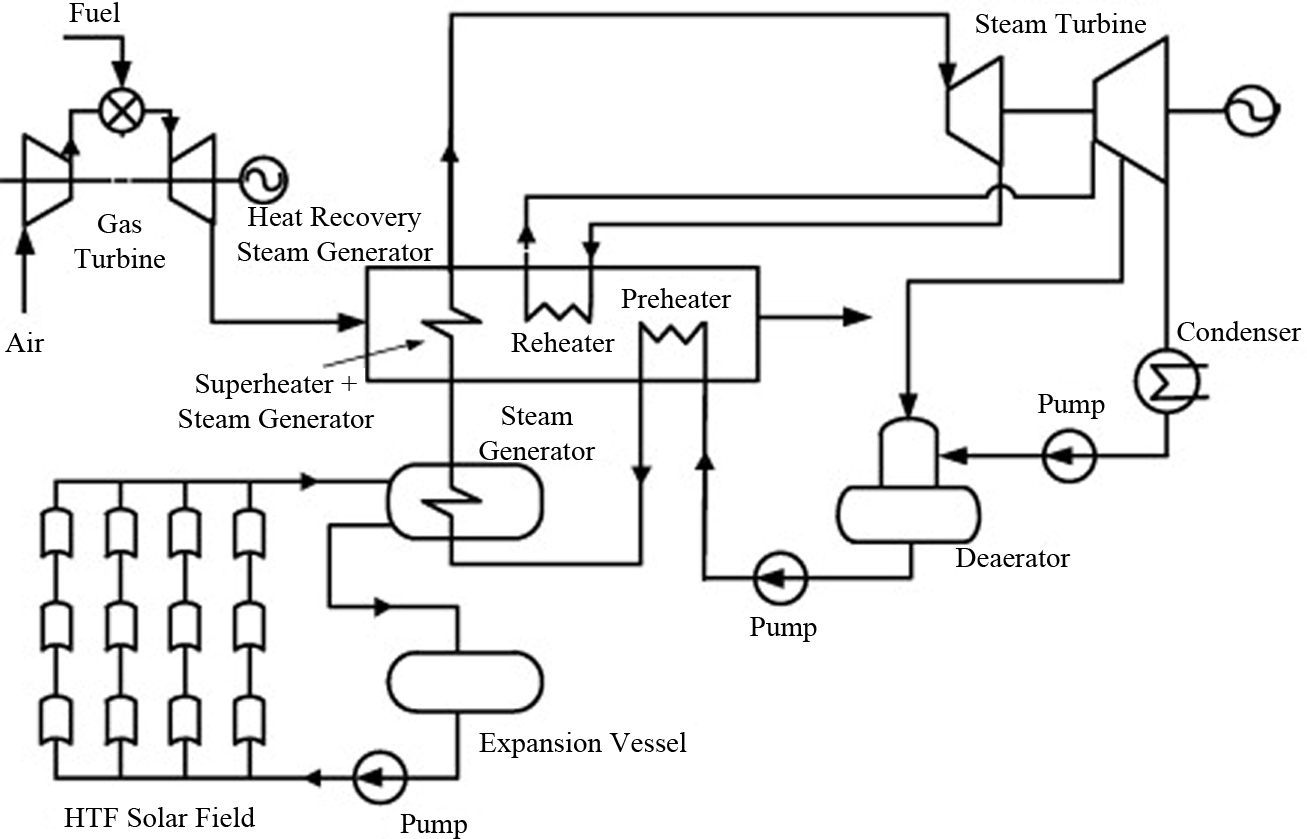
\includegraphics[width=.8\textwidth]{fig/Li2014.jpg}
\caption{将太阳能用于蒸发过程的ISCC系统结构示意图}
\label{fig:Li2014}
\end{figure}

G\"{u}len\cite{Gulen2015}使用了热力学第二定律中的㶲概念来简化ISCC系统的优化过程。经过㶲分析,为ISCC设计提供了基于物理方程的,对用户友好的指导方针。

Shaaban\cite{Shaaban2016}介绍了一种新型的ISCC系统,该系统同时考虑使用水工质朗肯循环(SRC)和有机工质朗肯循环(ORC)作为底部循环,其系统结构图如图\ref{fig:Shaaban2016}所示。有机工质循环用于冷却压缩空气,并利用这部分热量产生一部分电能。还研究了采用不同有机工质对该新型ISCC系统的性能的影响,结果表明使用R1234ze(z)作为有机工质可以在热力学,经济,安全和环境考虑之间取得较好的折衷。
\begin{figure}[!ht]
\centering
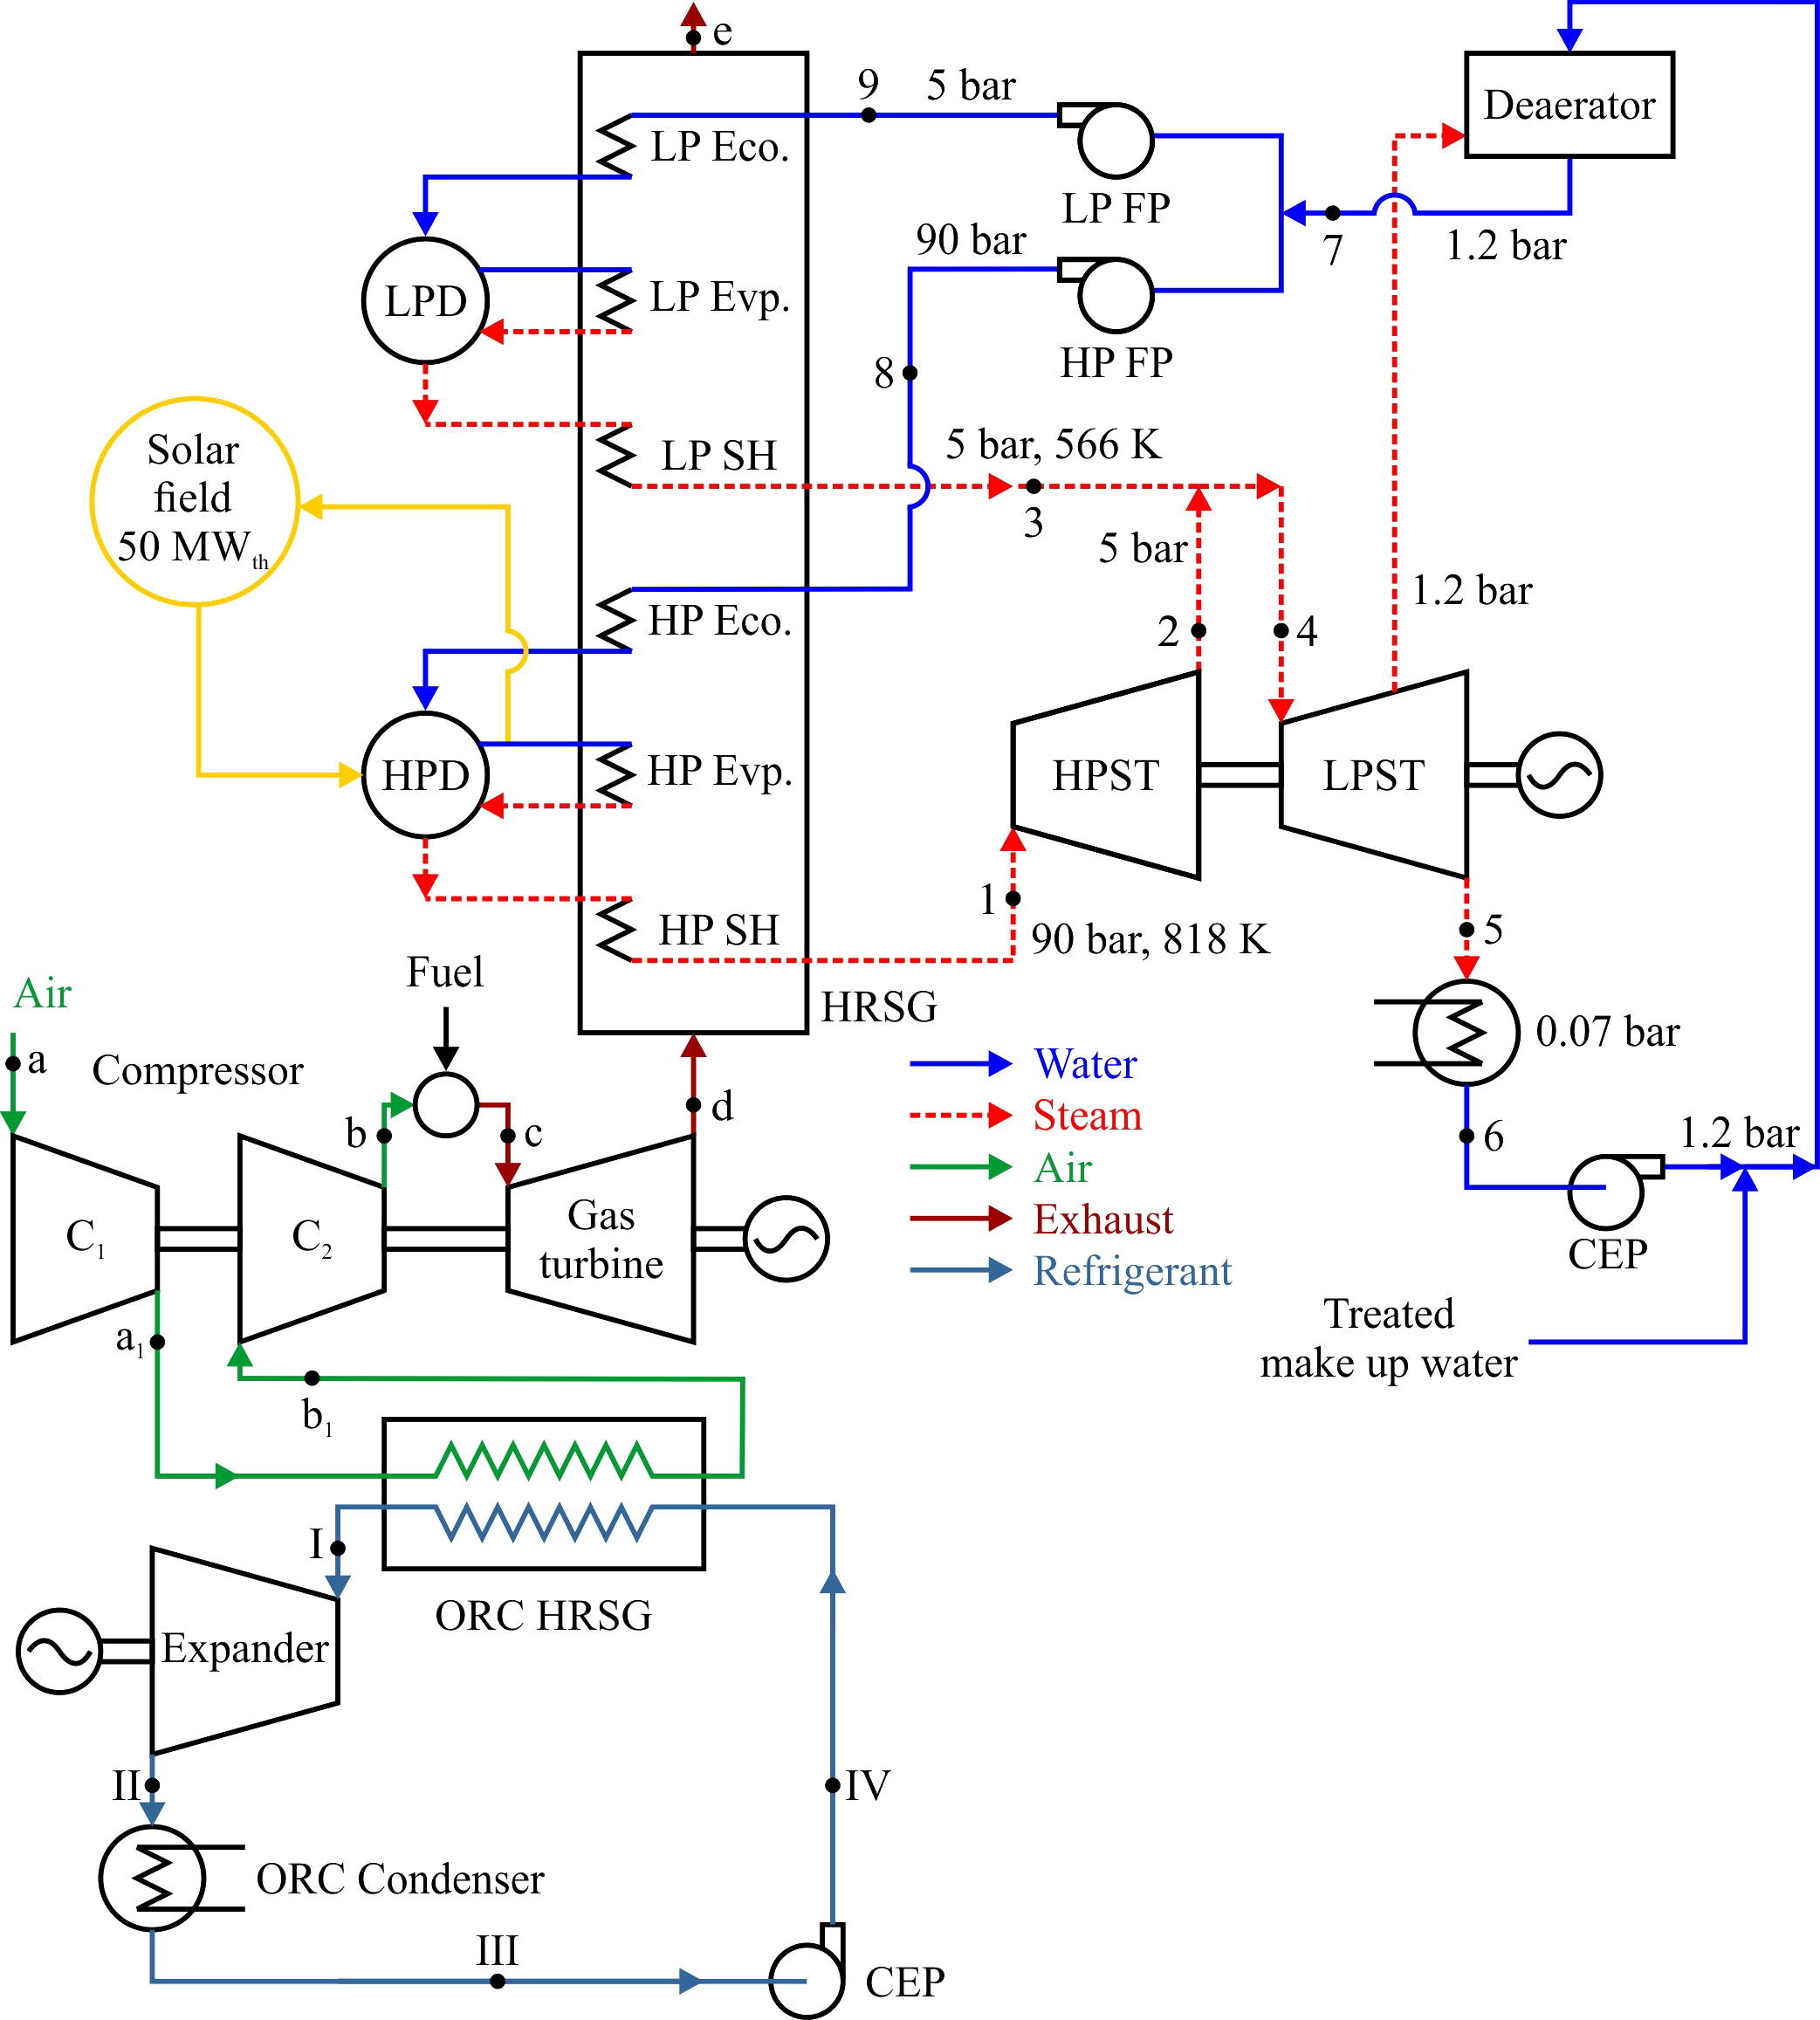
\includegraphics[width=.8\textwidth]{fig/Shaaban2016.jpg}
\caption{拥有两个底部循环的ISCC系统结构示意图}\label{fig:Shaaban2016}
\end{figure}

Alqahtani和Dalia\cite{Alqahtani2016}将ISCC电厂与独立CSP电厂、天然气联合循环电厂进行了对比分析。结果显示,将CSP整合进ISCC可以使发电成本比独立CSP电厂低35$\sim$40\%,并具有更好的调度能力。

Manente\cite{Manente2016}提出了一个具有三级压力的390$\,\mathrm{MWe}$的天然气联合循环,并以此评估不同集成方案的ISCC。为了得到最高的年平均效率和太阳能份额,分别进行了增大输出功率和节约燃料的操作策略。结果显示,节约燃料的操作策略所获得的年平均效率较低,这是因为燃气轮机的负荷下降导致系统整体效率下降。

Turchi等\cite{Turchi2014}提出了两种概念性的ISCC同槽式集热器混合设计的方案。在第一种方案中,燃气轮机的废气与在390$^\circ\mathrm{C}$以下运行的以导热油为传热流体的槽式集热器综合利用,在第二种方案中,燃气轮机的废气与在450$^\circ\mathrm{C}$以下运行的以熔融盐为传热流体的槽式集热器及TES(蓄热系统)一起综合利用。使用燃气轮机余热来补充TES的热量,这为系统提供了操作灵活性,同时提高了天然气利用效率。

Mukhopadhyay和Ghosh\cite{Mukhopadhyay2016}
提出了一种针对塔式太阳能电厂的热电联产梯级系统。该系统将传统燃气轮机的燃烧室用太阳能接收器替代,以布雷顿循环作为顶部循环,使用具有回热器的朗肯循环作为底部循环。

李晶等\cite{Li2016a}提出了一种新颖的梯级系统,该系统同时使用SRC和ORC。SRC采用对两相流体适应性高的螺杆压缩机实现膨胀做功。SRC的凝结热用于驱动ORC。

Al-Sulaiman\cite{AlSulaiman2014}分析了SRC-ORC联合循环采用不同种类的有机工质所能获得的输出功率。在联合循环中,SRC由槽式集热器提供热量,ORC由SRC的凝结热提供热量。结果表明,采用R134a的联合循环具有最佳㶲效率,其㶲效率可达26\%。

Dunham和Lipi\cite{Dunham2013}提出了综合布雷顿循环的分布式太阳能集热发电系统。通过对用于顶部布雷顿循环的工作流体和底部朗肯循环的工作流体进行分析后发现,使用CO$_2$的布雷顿顶部循环和使用R-245fa的朗肯循环底部循环的组合可以获得最高的组合循环效率(21.06\%),而单独的CO$_2$布雷顿循环在相同的工况下仅可达到15.31\%的峰值循环效率。

Bahrami等\cite{Bahrami2013}提出了一种联合有机工质朗肯循环。该朗肯循环用作斯特林循环的冷端散热器。有机工质循环的运行温度介于80$\mathrm{^\circ C}$到140$\mathrm{^\circ C}$之间。研究发现,联合循环的效率相比于独立的斯特林机可以提升4\%到8\%。

Thierry等\cite{Thierry2016}针对多级朗肯循环的两种不同结构提出了一种非线性求解方法。一种结构采用梯级利用的形式,一个循环作为顶部循环,另一个循环作为底部循环;另一种结构采用串联连接的形式让传热流体依次流经两个朗肯循环。经过对比分析发现,梯级结构可以获得比串联结构更高的效率,尤其是在热源温度较低的情况下。

Bahari等\cite{Bahari2016}考虑利用有机工质朗肯循环来回收利用斯特林机释放的热量。然而,该方案只是一个原始的设计方案,也没有考虑到将该方案应用于太阳能光热发电技术。

%\nomenclature[C]{LFC}{Linear Fresnel Collector}

\section{文献综述小结}
通过对前人研究工作的总结可以发现,太阳能光热发电技术正迎来高速发展的黄金期。大量的研究人员从实验研究、机理模型、数学方法等方面对太阳能光热发电技术进行了相关研究。然而,这些研究多是针对现有太阳能光热技术进行的改进性分析,也有文献提到了新的技术,比如空气槽式集热器、直接蒸汽发生系统等。但它们多是孤立地研究这些技术,没能将这些技术应用于光热发电系统(尤其是梯级光热发电系统)层面进行研究。此外,也有少量文献研究太阳能的梯级收集或梯级利用。然而,没有文献针对太阳能光热梯级系统进行系统性地分析,也没有文献提及在一个梯级系统中同时考虑能量的梯级收集与梯级利用。

\section{研究内容}
\label{sec:researchContent}

针对目前太阳能光热发电技术的特点,以及基于上述研究现状分析所存在的不足,本文以国家国际合作项目专项“太阳能梯级集热发电系统关键技术合作研究”为背景,目标是研究太阳能光热发电装置,利用各种传统型式的太阳能光热发电系统的优缺点以及热力特性,提出并组建,优化太阳能梯级集热发电系统,为探索出大规模低成本高效率利用太阳能的光热发电技术提供新的方案。主要研究内容包括:

\begin{enumerate}[label=(\arabic*)]
	
	\item 光热发电技术文献综述分析,对应于本文第一章。
	\setlength\parindent{2em}
	
	在简要介绍太阳能光热发电技术的研究背景及意义后,详细回顾了前人在已经商业应用的太阳能光热发电技术以及太阳能光热发电技术中的能量梯级收集利用领域所做的主要研究成果及研究现状,并简要概括了当前研究现状所存在的不足。
	\item 系统拓扑结构设计分析,对应于本文第二章。
	
	针对梯级系统拓扑结构的重要性及梯级发电系统结构选择的多样性,本文利用传统太阳能光热发电系统中各部件的特点,系统性地分析了太阳能梯级集热发电系统的拓扑结构中的多种方案,提出了多种采用梯级集热和梯级发电的太阳能梯级集热发电系统的拓扑结构方案。 

	\item 机理建模理论研究,对应于本文第三章。
	
	针对太阳能光热发电系统中关键部件的物理特性和运行机理,本文在关键部件的建模理论上进行深入研究。采用数学计算工具和系统开发工具,建立梯级系统中各部件的机理模型,进而组建梯级系统。采用面向对象的方法,充分利用封装、继承、多态等特性,保证各部件之间既具有独立性又具有关联性,同时保证系统中各模型易于替换和修改。最后开发了具有计算机软件著作权的太阳能光热发电系统设计软件。
	
	针对槽式集热器在长度方向上能量密度一致的特点,进行了整体换热系数沿长度方向均匀一致的假设,利用等热流密度下的流体与定温热源的传热计算公式,建立了槽式集热器的热效率计算模型。
	
	为碟式接收器建立了热网络模型,针对每一项热损失进行了详细地分析计算,通过求解热网络模型的各温度节点,得到碟式接收器的热效率计算模型。
	
	针对经典斯特林机模型考虑不可逆损失因素较少,计算误差较大的缺点,建立了考虑包括非理想换热、气体压力损失、活塞运动及摩擦损失、内部导热损失、穿梭导热损失等不可逆损失的斯特林机模型,并与经典模型和实验数据进行了对比分析。
	
	建立了\textbf{Stream}类用于部件的连接工作,部件的出口和入口用作连接的接口。两个不同的部件通过被赋值给同一个\textbf{Stream}对象而实现相互连接。以部件连接为基础实现了多部件间耦合计算功能。

	\item 斯特林机组排列方式优化研究,对应于本文第四章。
	
	考虑到斯特林机组不同排列方式对机组性能的影响,提出了五种基本的斯特林机组排列方式。利用太阳能光热设计系统建立了不同排列方式的斯特林机组仿真模型,并对其在不同影响因素下的性能进行了对比分析,找到了斯特林机组的最佳排列方式。

	\item 蒸汽发生系统的优化研究,对应于本文第五章。
	
	针对传统蒸汽发生系统在换热过程存在大量㶲损的缺点,本文提出了新型的分段加热系统,通过分段加热的方法来减少蒸汽发生过程中的温差,进而减少换热过程带来的㶲损,并降低太阳能场中传热流体的温度,提升太阳能场的集热效率。
	
	在新型的分段加热系统中,太阳能场别分成三个片区,分别为预热过程、蒸发过程和过热过程供热。可以通过调整各片区传热流体的流量,降低其对应的换热温差,降低各片区的传热流体的温度,提升集热效率,并降低换热过程的㶲损,提升太阳能光热系统的效率。

	\item 梯级系统评估分析研究,对应于本文第六章。
	
	给出了梯级系统的性能评估指标——整体光电转换效率,并提出了合适的独立系统方案进行对比分析。通过选取合理的系统参数,利用太阳能光热发电系统设计软件对梯级系统和其对应的独立系统进行了建模仿真分析。分析了不同因素对梯级系统的效率提升的影响,并得出了有利于梯级系统实施的条件。

	\item 太阳能梯级发电实验台的建设及实验研究,对应于本文第七章。
	
	参与了太阳能梯级发电实验台的建设工作及实验研究。针对晴天太阳辐射强度的不可控性、连续性及变化性,专门设计了特殊的实验工况来研究不同参数对槽式集热器和碟式集热器的集热效率的影响。明确了实验目的,设计了详细的实验步骤,并进行了相关的实验,获得了实验数据,并对建立的槽式集热器模型和碟式集热器模型进行了验证分析。
\end{enumerate}
\nomenclature[C]{CSP}{太阳能聚光集热发电}
\nomenclature[C]{HTF}{传热流体}